\Problem{Driving to Portland}{\PortDriveI}{
Discuss ``sensemaking'' with your group. Identify several ways of making sense of answers or contexts you have used in math or science courses.
}
\ProblemSub{\PortDriveA}{
(a) Identify several ways of making sense of answers or contexts you have used in math or science courses.
}
\Solution{\PortDriveASol}{

\begin{itemize}
	\item \textbf{Numerical Sensemaking:} Compare a numerical result against a reference number.
	\item \textbf{Unit Check:} Check the units of your expression to make sure they are what you expect. \\
	\textit{Example:} The units of $\beta$ must be $[\beta]=\frac{\text{gal}}{\text{h}^{2}}$ for $\beta t^{2}$ to have units of gallons.
	\item \textbf{Covariation:} See how changing the variables changes the output of your expression. See what the signs in your expression tell you. \\
	\textit{Example:} The minus sign in $G_{0}-\beta t^{2}$ tells us that the tank is getting emptier as time progresses (assuming $\beta > 0$), which we expect of a vehicle consuming gas as an energy source.
	\item \textbf{Special Case Analysis:} Choose values for variables which correspond to ``special cases,'' where the physical expectation is obvious and the math is simpler. \\
	\textit{Example:} We should have the most gas in the tank when we start, and if we plug in an initial time of $t=0$, we get $G(0) = G_{0}$. This tells us that $G_{0}$ is the initial amount of gas in the tank.
\end{itemize}
\textbf{IMPORTANT!} Do not just comment on the behavior of an expression without comparing to physical expectations. For example, do NOT just say ``$G(t)$ is decreasing, which makes sense.'' Say \textbf{why}: ``$G(t)$ is decreasing, which makes sense, as gas is consumed during travel.''
}
\ProblemSub{\PortDriveII}{
You are driving from Corvallis to Portland, and you measure how full your gas tank is (in gallons) as a function of time (in hours):
\[
G(t) = G_{0}-\beta t^{2}
\]
}
\ProblemSub{\PortDriveB}{
(b) Make sense of this expression with your group in as many different ways as you can, making use of as many different representations as you can.
}
\Solution{\PortDriveBSol}{

Multiple sensemaking examples are given in part (a). Additionally, we can learn a lot by looking at a visual representation. Let us graph the function:

\begin{figure}[h]
	\centering
	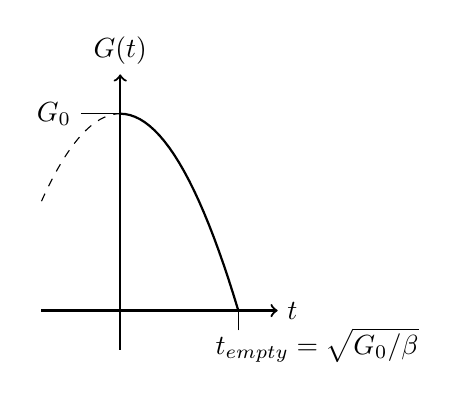
\begin{tikzpicture}
		\draw[thick,->] (0,-0.5) -- (0,3);
		\node[anchor=south] at (0,3) {$G(t)$};
		\draw (-0.5,2.5) -- (0,2.5);
		\node[anchor=east] at (-0.5,2.5) {$G_{0}$};
		\draw[thick,->] (-1,0) -- (2,0);
		\node[anchor=west] at (2,0) {$t$};
		\draw (1.5,-0.25) -- (1.5,0);
		\node[anchor=north] at (2.5,-0.1) {$t_{\text{empty}}=\sqrt{G_{0}/\beta}$};
		\draw[dashed, domain = -1:0, variable = \x]  plot ({\x},{2.5-10*\x*\x/9});
		\draw[thick, domain = 0:1.5, variable = \x]  plot ({\x},{2.5-10*\x*\x/9});
	\end{tikzpicture}
\end{figure}

There is a really important lesson here. Even if we provide you with an equation that is mathematically valid for all values of $t$, that does not mean it should be assumed to be an accurate model for all $t$.

For instance, $G(t)$ increases for $t<0$, which does not make sense while driving. The model probably should only be applied to $t>0$.

Furthermore, note that the slope gets steeper as $t$ increases. This tells us that gas is being consumed faster as time goes on. Should we expect fuel efficiency to vary like this?

Here is another very important question: when do we reach Portland? It is possible that we should have stopped graphing before $G(t)=0$ (out of gas). Graphing beyond the point at which the model applies may show us predictions that don't make sense.
}